\documentclass[a4paper,11pt,french]{article}
\usepackage[margin=2cm]{geometry}
\usepackage[thinfonts,latinmath]{uglix2}
\nouveaustyle
\begin{document}
\titre{Les fonctions}{Fiche Python}{\premiere}


Dans un programme, il est possible d'écrire des petits programmes, ou sous-programmes intermédiaires, appelés \textbf{fonctions}.\\
Une fonction est un programme qui porte un nom et utilise zéro, une ou plusieurs variables appelées \textbf{paramètres}.\\

\textbf{Syntaxe d'une fonction :}
\begin{pythoncode}
def nom_de_la_fonction(paramètre1,paramètre2,etc) :
   instruction(s)
   return resultat
\end{pythoncode}

\begin{remarque}[s]
	\begin{enumerate}[\textbullet]
		\item 	Si la fonction n’utilise aucun paramètre, on la définit de cette manière : \pythoninline{def nom_de_la_fonction() :}
		\item 	Le nom d’une fonction ne doit pas contenir d’espace. Les espaces peuvent être remplacés par des tirets \_ (sous le 8 sur le clavier).
	\end{enumerate}
\end{remarque}



\begin{tabular}{p{11cm}p{5cm}}
	\exo{}
	
	Une cuve de fuel est formée par deux parallélépipèdes. Les dimensions sont exprimées en m.
	
	Le volume de fuel contenu dans la cuve dépend de la hauteur du liquide.
	
	On a écrit ci-dessous le script de la fonction volume, qui retourne le volume de fuel en fonction de la hauteur de liquide.
	& \begin{center}
		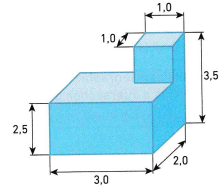
\includegraphics[width=4.5cm]{cuve}
	\end{center}
\end{tabular}

\begin{minipage}{6cm}
	\begin{pythoncode}
def volume(h) :
   if h < 2.5 :
      v = 6*h
   else :
      v = 12.5 + h
   return v
	\end{pythoncode}
\end{minipage}
\begin{minipage}{10cm}
	\begin{enumerate}[\bfseries 1.]
		\item 	Expliquer les calculs des lignes 2 et 3 du script.
		\item 	Expliquer le calcul de la ligne 5 du script.	
	\end{enumerate}
\end{minipage}


%\vspace{0.5cm}

\exo{}

La population d’un village était de 3 000 habitants en 2017. Chaque année, le village perd 2 \% de ses habitants. Le maire, qui est aussi informaticien, a écrit la fonction ci-dessous en langage Python.
\begin{pythoncode}
def population(annee) :
   pop = 3000
   for k in range(1, annee+1):
      pop = pop*0.98
   return pop
\end{pythoncode}

\begin{enumerate}[\bfseries 1.]
	\item 	Que renvoie la fonction \pythoninline{population} pour:
	\begin{enumerate}[\bfseries a.]
		\item 	un nombre d'anées égal à 1 ?
		\item 	un nombre d'années égal à 2 ?	
	\end{enumerate}
	\item 	Compléter le script ci-dessous pour qu’il calcule le nombre d’années à partir duquel la population du village sera inférieure ou égale à 1 500 habitants.
	\begin{pythoncode}
annee_seuil=0
pop = ....................................
while .................................... :
   anne_seuil = ....................................
   pop = population(annee_seuil)
	\end{pythoncode}
	\item tester ce script à l'ordinateur.
\end{enumerate}
\vspace{0.5cm}

\exo{}

Une patinoire propose deux formules de tarification :
\begin{enumerate}[\textbullet]
	\item 	\textbf{Formule A :} chaque entrée coûte 2,25 € ;
	\item 	\textbf{Formule B :} on paye un abonnement à l’année de 12 € et chaque entrée coûte 3,50 €.
\end{enumerate}
\begin{minipage}{9cm}
	Le directeur a écrit la fonction \pythoninline{tarifs} suivante :
	\begin{pythoncode}
def tarifs(entrees) :
   return entrees*5.25,12+3*entrees
	\end{pythoncode}
\end{minipage}
\begin{minipage}{1cm}
	\hspace{.5cm}\\
	
\end{minipage}
\begin{minipage}{7cm}
	\begin{enumerate}[\bfseries 1.]
		\item 	Que calcule la fonction \pythoninline{tarifs} ?
		\item 	Combien de valeurs la fonction \pythoninline{tarifs} renvoie-t-elle ?
		\item 	Utiliser cette fonction pour déterminer le nombre d’entrées nécessaires pour que la formule B soit plus avantageuse que la formule A.
	\end{enumerate}
\end{minipage}


\end{document}
